\chapter{从认知内核到完整 Agent}
\label{chap:from-cognitive-kernel-to-complete-agent}

\begin{chapteroverviewbox}
在前述 AgentOS 原理论中，我们已经建立了一个能够在固定功能拓扑上维持工作记忆、三相记忆、自我、生命周期生成倾向以及认知调节的持续主体。然而，到目前为止，这一主体仍主要被描述为一个“内部认知动力系统”。本章完成一个决定性的理论跃迁：我们不再把智能理解为封闭在认知内核中的计算过程，而把完整 Agent 定义为一个通过稳定的观测--行动边界持续嵌入现实的闭环系统。

本章的核心命题是：
\[
\boxed{
AgentSystem
=
AgentKernel
\bowtie
BodyRuntime
}
\]
其中，Agent Kernel 维持长期认知连续性、记忆、自我、目标与跨尺度决策；Body Runtime 则承担智能体与具体物理世界或数字世界之间的实时耦合。两者并非简单的“软件与硬件”关系，而是两个不同时间尺度、不同状态空间和不同职责域之间的动力学嵌合。

由此，Body 不再被限定为机器人机械身体。任何能够稳定地承载感知、行动、状态反馈并构成 Agent 与某一现实环境之间持续因果边界的系统，都可以成为 Agent 的 Body。机器人、汽车、浏览器、桌面操作系统、Shell、文件系统乃至由多个数字服务构成的操作环境，都可以在这一统一定义下成为不同形式的身体。

本章只建立这一跃迁所需的基础本体、边界和动力学关系。后续有关 Body Scale、统一身体接口、SGC、FCS、BPCC 与 Kernel--Body 适配机制的具体设计，将建立在本章给出的完整 Agent 定义之上。
\end{chapteroverviewbox}

\begin{figure}[htbp]
\centering
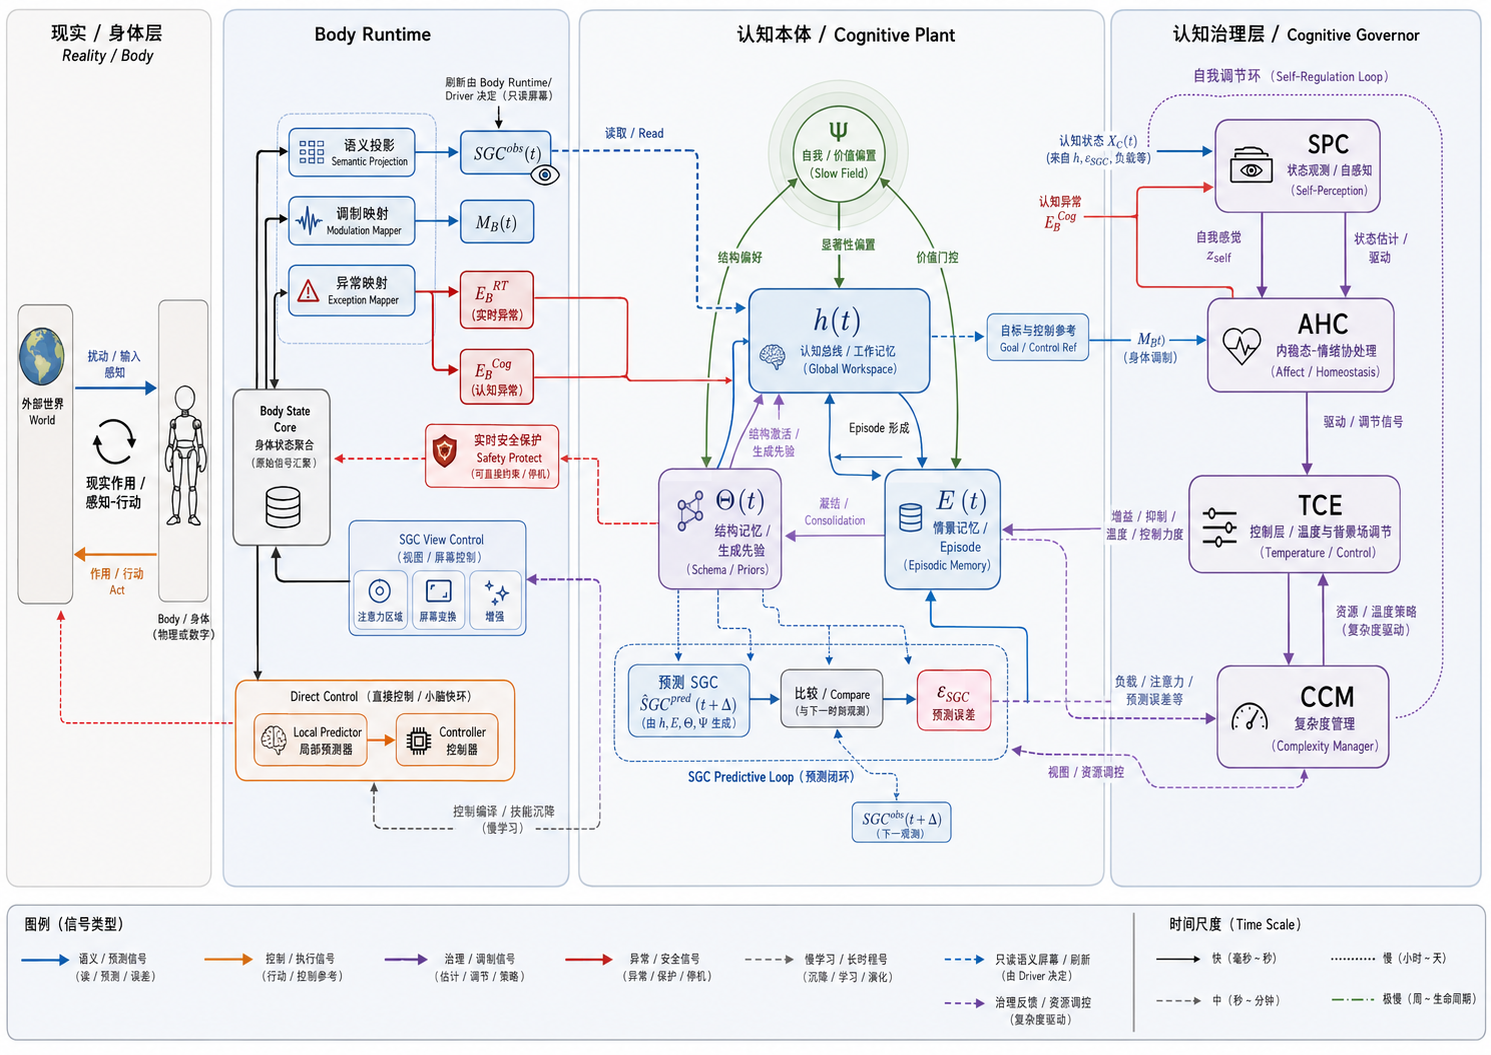
\includegraphics[width=.9\textwidth,height=.38\textheight,keepaspectratio]{images/cognitive-kernel-body-runtime.png}
\caption{Cognitive Kernel 与 Body Runtime 的完整主体}
\end{figure}
\section{无身体认知系统的理论边界}

在此前关于 AgentOS 的讨论中，我们已经可以构造一个相当完整的内部认知系统。设 Agent 的认知状态为
\[
\mathcal{X}_{C}(t)
=
\left[
h(t),
E(t),
\Theta(t),
\Psi(t),
\Omega(t),
G(t),
S_{\mathrm{self}}(t),
u_{\mathrm{cog}}(t)
\right],
\]
其中 $h$ 表示当前工作记忆状态，$E$ 表示情景经验轨迹，$\Theta$ 表示长期生成结构，$\Psi$ 表示相对稳定的身份与价值结构，$\Omega$ 表示更慢尺度的生命周期生成倾向，$G$ 表示当前目标结构，而 $S_{\mathrm{self}}$ 与 $u_{\mathrm{cog}}$ 分别表示自我状态估计与认知控制变量。从内部动力学上看，这个系统已经能够进行记忆召回、经验形成、结构学习、自我感知和目标驱动决策。若只观察其内部状态，我们甚至可以写出一个形式上完整的认知动力系统：
\[
\dot{\mathcal{X}}_{C}
=
F_{C}
\left(
\mathcal{X}_{C},
I_{C}
\right),
\]
其中 $I_C$ 是进入认知系统的输入。

然而，一个根本问题随即出现：如果 $I_C$ 只是由另一个软件模块提前准备好的符号输入，而认知系统产生的输出也只是某种待执行的符号，那么这个系统虽然拥有内部认知循环，却仍没有回答“主体如何真实存在于世界之中”的问题。其所有世界知识最终都必须依赖某个外部系统代替它完成感知，其所有行动意图也必须依赖另一个外部系统代替它进入现实。此时我们拥有的更准确地说是一个
\begin{statementbox}
CognitiveCore
\end{statementbox}
而不是一个闭合意义上的
\begin{statementbox}
Agent.
\end{statementbox}

这种差异不能简单理解为“有没有机械手”。真正缺失的是一个稳定的因果闭合。一个完整智能体必须使其内部状态能够通过行动影响现实，而现实变化又必须通过新的观测重新进入内部状态。因此最小闭环不是
\[
Input
\rightarrow
Reasoning
\rightarrow
Output,
\]
而应当是
\[
\boxed{
World_t
\rightarrow
Observation_t
\rightarrow
Cognition_t
\rightarrow
Action_t
\rightarrow
World_{t+1}
\rightarrow
Observation_{t+1}.
}
\]
只有后一种结构，系统的预测、判断和行动才能最终受到现实重新验证。否则，内部世界模型可能不断自洽，却不必与真实世界保持一致。

因此我们在这里引入一个重要区别：
\[
\boxed{
CognitiveClosure
\neq
WorldClosure.
}
\]
一个系统可以形成内部的认知闭环，例如
\[
h
\rightarrow
SPC
\rightarrow
TCE
\rightarrow
h',
\]
也可以形成记忆闭环：
\[
h
\leftrightarrow
E
\leftrightarrow
\Theta,
\]
但这些都不自动意味着系统与现实之间已经闭合。只有当行动必须重新经过现实，并由现实产生新的不可由内部模型直接伪造的观察结果时，我们才得到真正意义上的 World--Agent--World 闭环。

从控制论角度看，这意味着 Agent Kernel 本身并不是完整 Plant--Controller 系统。它更接近一个高层状态估计、规划与慢尺度控制结构。现实世界具有独立于 Agent 内部模型的状态：
\[
\mathcal{X}_{W}(t),
\]
而认知内核只能获得某种有限观测：
\[
y_t
=
O
\left(
\mathcal{X}_{W}(t)
\right)
+
\nu_t,
\]
其中 $\nu_t$ 表示观测噪声、不确定性与表示损失。Agent 进一步形成关于世界的内部状态估计：
\[
\hat{\mathcal{X}}_{W}^{A}(t),
\]
但原则上
\[
\boxed{
\hat{\mathcal{X}}_{W}^{A}(t)
\neq
\mathcal{X}_{W}(t).
}
\]
这一区别正是现实约束进入智能理论的数学入口。

因此，一个没有 Body Runtime 的认知内核面临三类基本边界。第一，它无法自行保证输入与现实具有可靠因果联系；第二，它无法自行保证行动意图真正改变了世界；第三，它无法可靠地区分“我预测行动成功”与“行动事实上已经成功”。换言之：
\[
\boxed{
ActionIntention
\neq
ActionExecution
\neq
ActionOutcome.
}
\]
这三者只有通过现实闭环才能被区分。

从智能动力学的角度，我们因此得到一个更严格的判断：持续智能并不只是“长期记忆加推理”，而是一个长期存在的结构必须不断在
\[
World
\rightarrow
Agent
\rightarrow
World
\]
这一闭环中维持自身。认知内核解决的是“主体内部如何形成连续认知”；Body 则解决“这个连续主体如何占据一个现实中的因果位置”。两者缺一不可。

这一结论也解释了为什么纯粹扩大模型参数并不能自然地产生完整 Agent。参数规模可以提高内部映射能力，却不能定义这个系统能够观测什么、能够改变什么、改变的速度是多少、哪些变化对自身具有不可逆代价，以及哪些现实结果具有最终解释权。所有这些问题都属于 Body 与现实耦合的问题。因此，从这一章开始，我们把“认知系统”与“完整智能体”严格区分，并把身体视为智能理论中的基础结构，而不是模型完成之后再附加的外围设备。

\section{Body 不是机器人：身体的功能本体定义}

当我们第一次把 Body 引入 AgentOS 时，最容易出现的误解是把 Body 直接等同于机器人机械结构。例如，把摄像头看成眼睛，把机械臂看成手，把轮式底盘看成腿，然后认为只有具有这些物理部件的 Agent 才是具身智能。这种定义对于机器人学而言具有直观性，但对于通用 AgentOS 来说过于狭窄。因为从智能动力学的角度，我们真正关心的不是一个载体是否“长得像身体”，而是它是否建立了主体与现实之间稳定的观测--行动因果边界。

因此我们将 Body 定义为：
\[
\boxed{
Body
=
ControlledAndSensedCarrierOfAgency.
}
\]
即：
\begin{statementbox}
身体是主体能够持续感知、持续控制，并借此对某一现实环境施加因果影响的承载结构。
\end{statementbox}

这个定义包含三个不可缺少的条件。第一是 \emph{sensed}，即 Agent 必须能够获得关于 Body 及其环境的状态反馈；第二是 \emph{controlled}，即 Agent 的内部决策能够通过该结构影响现实；第三是 \emph{persistent carrier of agency}，即这种感知与控制关系在时间上足够稳定，使主体可以建立连续的“我能够通过什么方式影响世界”的结构模型。

我们可以将其形式化。设某一候选 Body 的内部状态为
\[
x_B(t)\in\mathcal X_B,
\]
其可感知输出为
\[
y_B(t)
=
H_B
\left(
x_B(t),
x_W(t)
\right),
\]
Agent 可以施加控制输入
\[
u_B(t)\in\mathcal U_B,
\]
而其状态演化满足
\[
\dot{x}_B
=
F_B
\left(
x_B,
x_W,
u_B
\right).
\]
如果存在稳定映射
\[
\mathcal O_B:
(x_B,x_W)
\rightarrow
y_B
\]
和
\[
\mathcal A_B:
u_B
\rightarrow
\Delta(x_B,x_W),
\]
使 Agent 能够持续通过 $y_B$ 感知现实，并通过 $u_B$ 对现实产生可归因的影响，那么该系统就满足 Body 的最低功能条件。

因此 Body 的本体身份并不取决于材料：
\[
\boxed{
BodyOntology
\perp
Substrate.
}
\]
金属、硅、电子设备、软件进程甚至某些受控网络服务，在满足上述因果关系时都可以成为身体的一部分。这里体现的是我们在认识论部分已经建立的一个基本原则：同类智能不应由实现材料分类，而应依据功能闭环、语义结构与多尺度动力关系进行判断。

这一点同时说明，Body 不能简单定义成“Agent 能调用的全部工具”。工具与身体之间存在重要差异。一个偶尔调用的外部服务不一定属于 Body。若 Agent 调用一个天气 API，API 更适合被理解成 Tool；而如果一个系统持续向 Agent 提供自身状态，具有稳定控制接口，并成为 Agent 行动闭环的一部分，那么它可能逐渐具有 Body 的功能属性。因此，Body 与 Tool 之间不是纯粹二元分类，而存在一个由持续性、控制深度、状态反馈和主体归属感共同决定的谱系。

可以概念性定义 Body Coupling Strength：
\[
\kappa_B
=
F
\left(
C_{\mathrm{observe}},
C_{\mathrm{control}},
P_{\mathrm{continuity}},
I_{\mathrm{identity}},
R_{\mathrm{feedback}}
\right),
\]
其中 $C_{\mathrm{observe}}$ 表示可观测程度，$C_{\mathrm{control}}$ 表示可控制程度，$P_{\mathrm{continuity}}$ 表示耦合持续性，$I_{\mathrm{identity}}$ 表示该载体是否被纳入主体持续状态，$R_{\mathrm{feedback}}$ 表示行动结果是否稳定回流。$\kappa_B$ 越高，一个载体就越接近 Agent 的身体；越低，则越接近偶发工具或外部资源。

这一连续谱十分重要，因为未来 Agent 很可能同时拥有多种身体。例如，一个持续数字 Agent 可以长期拥有桌面操作环境，同时临时接管一台移动机器人，又通过网络控制家庭设备。在这种情况下，如果坚持“一 Agent 对应一具机械身体”，理论会立即失效。更准确的是：
\[
\boxed{
Agent
\rightarrow
\{Body_1,Body_2,\ldots,Body_n\}
}
\]
而不同 Body 可以在不同时间拥有不同的有效控制权和感知权。

但是，这并不意味着主体也随 Body 分裂。我们此前已经建立了单一持续主体原则。因此：
\[
\boxed{
OnePersistentSubject
\not\Rightarrow
OnePhysicalBody.
}
\]
同一个 Agent 可以拥有多个身体，却仍维持单一的 $h/E/\Theta/\Psi/\Omega$ 生命周期结构。真正连续的是主体，而不是某一套具体传感器或执行器。

这一理论转变还有一个更深的含义：Body 实际上定义了 Agent 的现实边界。没有身体时，“世界”只是一个输入集合；有了 Body 后，世界出现了可达性结构。一扇门对于具有机械臂的机器人与没有机械臂的机器人不是同一个功能世界；文件系统对于能够执行文件操作的数字 Agent 与只能阅读文本的 Agent 也不是同一个功能世界。因此，Body 不只是输入输出接口，而是在事实上决定：
\[
\boxed{
WhatCanBeObserved,\quad
WhatCanBeChanged,\quad
WhatCanBeReached.
}
\]
换言之，Body 定义了 Agent 的 \emph{actionable reality}。

因此，本书之后所说的具身，不应被狭义理解为“拥有类人生理形态”，而应理解为：
\[
\boxed{
Embodiment
=
PersistentCausalEmbeddingIntoAnEnvironment.
}
\]
这个定义同时覆盖物理机器人与数字 Agent，也为后续建立统一 Body Scale、语义现实表示和快速身体控制提供了共同本体基础。

\section{物理 Body：进入连续物理世界的因果承载}

物理身体是 Body 概念最直观的实例，也是我们检验完整 Agent 理论最严格的现实环境。一个物理机器人并不是简单地把摄像头图像传给 Agent Kernel，再把语言模型生成的动作指令发送给电机。真实物理世界具有连续时间、高频扰动、动力学惯性、执行延迟、能量约束以及不可逆风险。因此，当认知内核进入物理世界时，它面对的是一个与语言推理完全不同的状态空间。

设物理 Body 状态为
\[
x_B(t)
=
[
q(t),
\dot q(t),
e(t),
T(t),
s(t),
r(t),
\ldots
],
\]
其中 $q$ 与 $\dot q$ 可以表示机械构型和速度，$e$ 表示能源状态，$T$ 表示温度等设备状态，$s$ 表示传感器状态，$r$ 则可以表示局部风险和资源余量。外部环境状态为
\[
x_W(t).
\]
物理系统整体演化满足
\[
\dot{x}_B
=
F_B
\left(
x_B,
u_B,
x_W,
d_B
\right),
\]
其中 $u_B$ 是控制输入，$d_B$ 是未建模扰动。

认知内核不可能，也不应该，在每一个物理控制周期中直接处理完整 $x_B$。如果一个关节控制器以 $1\,\mathrm{kHz}$ 运行，而高层认知周期在秒级甚至更慢，那么：
\[
\tau_{\mathrm{servo}}
\ll
\tau_{\mathrm{cognition}}.
\]
让 Agent Kernel 在每一个 servo timestep 上决定电流或扭矩，不仅低效，而且会破坏实时性。因此，物理 Body 天然要求多尺度闭环：
\[
\boxed{
FastLocalLoop
\subset
SlowGlobalLoop.
}
\]

这与我们前面关于智能频谱的认识完全一致。高层智能并不需要“管理所有细节”，而应定义较慢尺度上的目标、约束和可行区域；低层系统则在这些约束内部完成快速稳定控制。于是：
\[
\boxed{
HigherLevelSetsFeasibleRegion,
\qquad
LowerLevelOptimizesInsideIt.
}
\]
例如，认知内核可以决定“把这个杯子安全放到桌面指定区域”，但不应逐毫秒指定每个电机的控制量。后一过程属于身体内部快速闭环，而高层只需要获得足以判断任务进展、异常和结果的结构化反馈。

由此我们得到一个重要状态分离：
\[
\boxed{
BodyState(t)
\neq
h(t).
}
\]
工作记忆 $h(t)$ 是当前需要全局显式处理的认知结构，而 BodyState 是身体真实运行所需的高频状态。两者之间可能存在映射，但绝不能等同。如果 Body 的所有内部状态都进入 $h$，工作记忆有限容量定理将立即被底层噪声和高频变量击穿。

因此，物理身体实际上成为认知复杂度的第一道屏障。大量可局部解决的扰动，应当在 Body 层被吸收：
\[
Disturbance
\rightarrow
LocalBodyLoop
\rightarrow
Correction,
\]
而不是：
\[
Disturbance
\rightarrow
h
\rightarrow
GlobalReasoning.
\]
只有当局部控制无法解释或处理某种残差时，相关结构才应该向上升级：
\[
\varepsilon_B
>
\theta_B
\quad\Rightarrow\quad
Escalation.
\]
这正是后来“Normal Dynamics Stay Local”和“Predict Locally, Escalate Residual Globally”原则的起点。

物理 Body 还带来了一个纯认知系统中很容易被忽略的问题：行动具有代价。语言模型生成一个错误 token，通常可以在下一轮纠正；机械系统执行一个错误动作，则可能造成碰撞、损坏或不可逆环境改变。因此，物理 Body 的行动空间应表示成带约束的可行集合：
\[
u_B(t)
\in
\mathcal U_{\mathrm{safe}}
\left(
x_B,
x_W
\right),
\]
其中
\[
\mathcal U_{\mathrm{safe}}
\subseteq
\mathcal U_B.
\]
这意味着 Agent 的自由行动空间从一开始就必须受到物理可行性、安全性和能力边界的约束。

此外，身体本身会变化。电池下降、关节磨损、传感器漂移、负载变化、温度上升，都会使同一个高层动作产生不同的实际结果。因此 Agent 不只是“通过身体控制世界”，还必须逐渐学习：
\begin{statementbox}
WhatThisBodyCanCurrentlyDo.
\end{statementbox}
这意味着身体状态是 Agent 世界模型的一部分，并且 Body Capability 并不是常数：
\[
\mathcal C_B
=
\mathcal C_B(t).
\]
一个成熟智能体必须持续估计自己的能力边界，而不是假设“曾经做得到的事情永远做得到”。

这一点与自我理论存在深刻联系。$\Psi$ 描述“我是谁”主要位于慢认知结构层，而 Body 描述“我现在通过什么载体进入现实”。两者不能混为一谈，但也不能完全分离。一个 Agent 换了一具身体，可能仍然保持身份连续；但新的身体会逐渐改变其行动经验、技能结构和未来发展空间。因此：
\[
\boxed{
IdentityContinuity
\neq
BodyIdentity,
}
\]
同时：
\[
\boxed{
BodyHistory
\rightarrow
Experience
\rightarrow
SelfDevelopment.
}
\]

物理 Body 因此不是认知内核的外围执行器，而是 Agent 生命周期的因果组成部分。一个真正长期存在的具身智能体，其自我、能力和经验必然在与具体身体的长期耦合中逐渐形成。这也解释了为什么未来 AgentOS 不能只研究“怎样让模型控制机器人”，而必须研究身体状态、认知状态、局部控制与长期记忆之间如何形成稳定的多尺度动力系统。

\section{数字 Body：数字世界同样可以构成真实具身环境}

如果我们接受 Body 的功能本体定义，那么一个很重要的结论自然出现：具身智能并不只存在于物理空间。对于一个主要工作在数字环境中的 Agent，操作系统、浏览器、文件、应用程序、网络服务和数字身份共同组成了其能够持续感知并施加行动的现实环境。因此，一个数字 Agent 同样可以拥有严格意义上的 Body。

设数字环境状态为
\[
x_D(t)
=
[
W(t),
P(t),
F(t),
N(t),
A(t),
S(t),
\ldots
],
\]
其中 $W$ 表示窗口/界面状态，$P$ 表示进程状态，$F$ 表示文件系统，$N$ 表示网络状态，$A$ 表示应用程序状态，$S$ 表示权限或安全状态。一个数字 Agent 能够通过观察接口获得
\[
y_D(t)
=
O_D(x_D(t)),
\]
并通过一组动作
\[
u_D(t)
\in
\mathcal U_D
\]
改变该环境：
\[
x_D(t+1)
=
F_D
\left(
x_D(t),
u_D(t),
\eta_t
\right),
\]
其中 $\eta_t$ 表示其他程序、用户、网络和外部服务造成的环境变化。

从这一形式看，数字环境与物理环境在 Agent 的抽象层上具有完全相同的结构：
\[
\boxed{
Observe
\rightarrow
Model
\rightarrow
Act
\rightarrow
NewState.
}
\]
区别主要在于具体动力学。物理世界通常具有连续状态、惯性和力学约束；数字世界更多表现为混合离散--连续状态、协议约束、权限边界和事务逻辑。但是这并不削弱数字环境的现实性。对于一个数字 Agent 来说，删除一个文件、发送一封邮件、修改数据库记录、提交一段代码，都是具有真实因果后果的行动。

因此，我们不能把“数字 Agent”理解为一个没有身体的 Agent。更准确地说，它具有：
\begin{statementbox}
DigitalBody.
\end{statementbox}
其身体不是机械肢体，而是由操作接口、权限系统、持续数字状态和执行能力共同组成。

这个观点对于 AgentOS 尤其重要，因为它意味着我们无需等待通用人形机器人出现，便可以首先在数字环境中验证许多 Body 理论。例如，数字 Agent 是否能够形成稳定的行动技能；是否能够区分预测状态和实际执行结果；是否能够维护身体/环境能力模型；是否能够在低层操作失效时把异常重新提升到认知层；是否能够在不同数字 Body 之间实现能力迁移。这些问题都可以先在 Browser、Desktop、Shell 等环境中进行研究。

数字 Body 也具有自身的“身体状态”。例如：
\[
\fitdisplay{
x_D^{body}
=
[
Permission,
Connectivity,
ApplicationAvailability,
Storage,
Compute,
CredentialState,
SessionState
].
}
\]
这些状态与人类身体的能量、温度或损伤不同，但在功能上具有类似意义：它们限制 Agent 当前能够执行哪些动作。如果某个 API token 失效，Agent 的行动能力会下降；如果网络断开，外部服务变得不可达；如果文件系统只读，某些计划无法执行。因此数字 Agent 同样需要回答：
\begin{statementbox}
WhatCanIDoNow?
\end{statementbox}
而不只是：
\[
WhatDoIWantToDo?
\]

进一步地，数字世界中的权限系统可以被理解为一种显式 Body Boundary。某个 Agent 可能具有：
\[
Read(File),
\qquad
Write(File),
\qquad
Execute(Process),
\qquad
Send(Message),
\]
但不具备：
\[
Delete(SystemFile).
\]
因此其可行动空间同样满足：
\[
\mathcal U_D^{A}
\subset
\mathcal U_D.
\]
这与物理身体的力学能力边界具有功能同构。

数字 Body 还使“身体可替换性”表现得更加清楚。同一个 Agent 可以从 Browser Body 切换到 Shell Body，或者从桌面操作环境切换到移动设备环境。它的长期记忆、自我和目标可以保持，而底层交互方式发生变化。因此：
\[
\boxed{
AgentIdentity
\neq
InterfaceIdentity.
}
\]
这为我们后面讨论 Body Scale 提供了最直接的工程实验条件：一个成熟 Agent 应该能够最大程度地保留关于任务、对象、目标和策略的高层 CSO，而只重新学习“这个新身体怎样观察和行动”。

数字具身还使一个长期以来模糊的问题变得明确：Computer Use Agent 并不是“语言模型调用 GUI 工具”的简单组合。如果系统能够维持持续主体、持续环境状态、操作历史、行动能力模型以及动作--反馈闭环，那么 Computer Use 本身已经构成一种完整的具身智能实验场。也正因此，在我们的工程路线中，数字身体可以成为 AgentOS 最早的现实验证平台，而不只是人形机器人之前的廉价替代品。

从理论上讲，物理 Body 与 Digital Body 可以统一写成：
\[
\boxed{
Body_i
=
(
\mathcal X_i,
\mathcal O_i,
\mathcal U_i,
\mathcal D_i,
\mathcal C_i
),
}
\]
其中 $\mathcal X_i$ 是身体与环境状态空间，$\mathcal O_i$ 是可观测映射，$\mathcal U_i$ 是动作空间，$\mathcal D_i$ 是动力学/状态转移结构，$\mathcal C_i$ 是约束集合。这样，我们就获得了一个与材料无关的身体定义，也为真正跨物理--数字世界的通用 AgentOS 建立了统一数学入口。

\section{Browser、Shell 与 Filesystem 也是身体的一部分}

在数字 Body 的一般定义之上，我们可以进一步分析几个最典型的数字身体结构：Browser、Shell 与 Filesystem。表面上，它们似乎只是 Agent 使用的三种 Tool；但当它们成为持续 Agent 与数字现实之间高频、稳定、可观测、可控制的主要因果接口时，它们便开始具有 Body 的功能属性。

首先考虑 Browser。普通软件意义上的浏览器是一个应用程序；但对 Computer Use Agent 而言，浏览器实际上提供了一个持续数字空间。其状态不仅包括网页文本，还包括：
\[
\fitdisplay{
x_{\mathrm{browser}}
=
[
DOM,
Viewport,
Tabs,
History,
Cookies,
Session,
Forms,
Downloads,
Permissions,
NetworkState
].
}
\]
Agent 可以观察这一状态的某些投影，并通过点击、输入、滚动、导航等动作改变它。于是存在：
\[
O_{\mathrm{browser}}
:
x_{\mathrm{browser}}
\rightarrow
y_{\mathrm{agent}}
\]
与
\[
A_{\mathrm{browser}}
:
u_{\mathrm{agent}}
\rightarrow
\Delta x_{\mathrm{browser}}.
\]
如果这一关系持续存在，那么 Browser 对该 Agent 而言就不仅是一个工具，而是其进入 Web Reality 的一种数字身体。

更重要的是，浏览器中的“世界”不是纯粹视觉画面。一个按钮具有位置、文本、可点击性、权限状态、当前交互上下文和潜在后果。因此 Agent 真正需要的不是像素本身，而是：
\begin{statementbox}
ActionableDigitalReality.
\end{statementbox}
这与物理机器人需要的可行动三维现实本质一致，只是坐标空间不同。

Shell 更能体现数字 Body 的执行属性。通过 Shell，Agent 可以直接作用于操作系统状态：
\[
Process,
File,
Network,
Package,
Service,
Permission.
\]
Shell action 可表示为：
\[
u_{\mathrm{shell}}
=
(Command,Arguments,Environment,Privilege).
\]
执行结果则形成：
\[
y_{\mathrm{shell}}
=
(ReturnCode,Stdout,Stderr,StateChange).
\]
这已经是非常标准的 Action--Reality--Observation 闭环。如果 Agent 只生成 shell command，却从不读取实际 return code 与状态变化，那么它只是在“想象行动”；只有结果重新进入 Agent 状态时，行动才真正完成闭合。

Filesystem 则具有更特殊的位置，因为它同时表现出 Body Environment 与 External Memory 的双重性质。从环境角度，它是 Agent 可以改变的数字现实：
\[
Write(File)
\Rightarrow
WorldState'.
\]
从记忆角度，它又可以承载被外化的 Agent-CSO，使未来认知重新恢复某些结构：
\[
AgentCSO
\rightarrow
File
\rightarrow
FutureAgentCSO.
\]
因此 Filesystem 是 Body 与 Memory 两种理论之间的重要交叉结构。

这提醒我们，AgentOS 中的组件不能只通过静态名词分类。一个实体的理论角色取决于它与主体形成什么功能关系。某个 File 可以是：
\[
ExternalMemory,
\]
也可以是：
\[
EnvironmentState,
\]
还可能是：
\[
ActionTarget.
\]
同一个 Browser 可以在一次任务中只是 Tool，在长期持续操作中则成为 Body Runtime 的核心组成部分。

因此，我们更适合用关系而不是物品本身来定义 Body membership。可以引入：
\[
M_B(r,t)
\in
[0,1],
\]
表示资源 $r$ 在时刻 $t$ 被纳入 Body 的功能程度。其值由：
\[
M_B
=
F(
Observability,
Controllability,
Continuity,
FeedbackDensity,
IdentityIntegration
)
\]
决定。

于是，一个长期运行的桌面 Agent 可能具有：
\[
M_B(\mathrm{Browser})\approx1,
\]
\[
M_B(\mathrm{Shell})\approx1,
\]
而某个偶尔使用一次的远程 API 可能只有：
\[
M_B(\mathrm{API})\ll1.
\]

这一连续定义避免了“Tool 与 Body 到底如何二分”的伪问题。真正需要研究的是：哪些外部结构已经被 Agent 纳入了其持续观测--行动闭环。

此外，Browser、Shell 与 Filesystem 共同说明数字 Body 并不是一个单一接口，而更像一个多执行器、多感知通道的复合身体。可以写成：
\[
Body_D
=
B_{\mathrm{browser}}
\cup
B_{\mathrm{shell}}
\cup
B_{\mathrm{filesystem}}
\cup
B_{\mathrm{network}}
\cup
\cdots
\]
但这些接口不能各自独立地代表主体。真正主体仍由 Agent Kernel 的持续生命周期状态维持。Body 只定义主体当前能够通过哪些路径进入现实。

这一关系与人类也具有结构上的相似性：眼、手、语言、工具并不是“主体本身”，但它们共同决定主体可以怎样观察和改变世界。数字 Agent 的 Browser、Shell 和 Filesystem 虽然材料完全不同，却可以在功能层实现相似的因果结构。

因此，本章在数字环境中的一个重要结论是：
\begin{conclusion}
数字具身不是比物理具身低一级的模拟；它是另一种真实的 Agent--World 因果嵌入。
\end{conclusion}
其现实约束不是重力和惯性，而更多表现为协议、权限、事务、网络状态和软件逻辑。但只要行动具有真实后果、状态具有持续性、反馈能够重新约束 Agent，数字世界就足以构成完整的具身环境。

\section{Cursor 作为数字末端执行器}

为了进一步理解数字 Body，我们可以把 Cursor 看成一个极具代表性的结构。它不是因为视觉上像“手”才重要，而是因为它在图形界面中承担了从高层行动意图到局部环境状态改变之间的最终执行映射。因此，在数字具身中，Cursor 可以被形式化为一种：
\begin{statementbox}
DigitalEndEffector.
\end{statementbox}

在机器人控制中，一个机械臂末端执行器的状态可以表示为：
\[
x_{ee}
=
(p,R,v,\omega,\ldots),
\]
其动作影响世界中的接触、抓取和操作。同样，在 GUI 环境中，Cursor 具有位置：
\[
p_c=(x_c,y_c),
\]
动作集合：
\[
\mathcal U_c
=
\{
Move,
Click,
DoubleClick,
Drag,
Scroll,
Hover
\},
\]
并通过这些动作改变界面状态：
\[
x_{GUI}(t+1)
=
F_{GUI}
\left(
x_{GUI}(t),
u_c(t)
\right).
\]

因此，高层任务：
\[
\text{“提交这份表单”}
\]
并不能直接作用现实。它必须逐步被映射成：
\[
Goal
\rightarrow
InterfaceObject
\rightarrow
TargetRegion
\rightarrow
CursorTrajectory
\rightarrow
Click
\rightarrow
GUIStateChange.
\]
这与物理机器人中的：
\[
Goal
\rightarrow
ObjectPose
\rightarrow
EndEffectorTrajectory
\rightarrow
Contact
\rightarrow
WorldStateChange
\]
在功能结构上高度一致。

这并不意味着 GUI 控制和机械控制具有相同动力学，而意味着它们共享：
\[
\boxed{
HighLevelIntent
\rightarrow
EmbodiedActionCoordinates
\rightarrow
RealityTransition
}
\]
这一抽象结构。

Cursor 的例子特别有助于说明 AgentOS 为什么需要将“认知动作”与“身体动作”分离。认知层适合表示：
\[
Click(
SubmitButton
),
\]
而不是：
\[
MoveCursorTo(824,517).
\]
前者是语义动作，后者是具体身体动作。若整个 AgentOS 绑定于像素坐标，则换一个分辨率、窗口布局或设备后，高层能力会大幅失效。真正通用的 Agent 应保留：
\begin{statementbox}
SemanticActionInvariant
\end{statementbox}
并把具体坐标映射留给身体侧。

我们可以表示：
\[
a^{semantic}
=
Click(Entity_i),
\]
而具体执行为
\[
a^{body}
=
\phi_B
\left(
a^{semantic},
x_B
\right).
\]
其中 $\phi_B$ 是当前 Body 对语义动作的具体实现映射。

对于 Desktop Body：
\[
\phi_{\mathrm{desktop}}
:
Click(Button_i)
\rightarrow
CursorTrajectory+MouseClick.
\]
对于触摸屏 Body：
\[
\phi_{\mathrm{touch}}
:
Click(Button_i)
\rightarrow
Touch(x_i,y_i).
\]
对于浏览器 DOM 接口：
\[
\phi_{\mathrm{DOM}}
:
Click(Button_i)
\rightarrow
DOMEvent(i).
\]
尽管身体实现完全不同，高层 Agent-CSO：
\[
\boxed{
Click(TargetEntity)
}
\]
可以保持相对稳定。

这正是后面 Body Scale 原理的一个重要前提：通用智能的扩展能力不只取决于“会不会某个动作”，还取决于该动作的语义结构能否跨 Body 保留。换句话说：
\[
\boxed{
ActionMeaning
\neq
ActionImplementation.
}
\]

Cursor 还揭示了动作反馈的必要性。如果 Agent 移动并点击 Cursor 后，只根据自己的动作命令推断“按钮已经被点击”，就会产生：
\[
ActionIssued
\Rightarrow
AssumedSuccess.
\]
这是错误的。现实中可能发生窗口移动、按钮禁用、点击被遮挡、网络失败或应用程序无响应。因此动作后必须重新读取：
\[
x'_{GUI},
\]
然后判断：
\[
Success
=
Verify(
Goal,
x'_{GUI}
).
\]
于是完整结构为：
\[
\boxed{
Intent
\rightarrow
CursorAction
\rightarrow
GUIReality
\rightarrow
Observation
\rightarrow
Verification.
}
\]

这与我们在整个 AgentOS 理论中反复坚持的：
\begin{statementbox}
RealityIsUltimateConstraint
\end{statementbox}
完全一致。

因此，Cursor 虽然只是一个非常小的数字接口，却已经呈现出 Body Runtime 的核心逻辑：高层意图必须被转换成某一身体特定的动作坐标；动作必须经过现实；现实结果必须重新被观测；异常必须能够触发新的认知。正是在这个意义上，一个光标、一个机械臂末端和一个车辆方向控制系统可以被放进同一个更一般的身体理论中进行研究。

\section{完整 Agent 的统一动力学定义}

经过前面的分析，我们现在可以正式给出本书意义上的完整 Agent 定义。一个完整 Agent 不再等同于模型、不等同于认知内核，也不等同于机器人身体，而是一个由持续认知主体、具体身体运行时以及现实环境共同组成的闭环动力系统。

首先定义：
\[
\boxed{
AgentSystem
=
AgentKernel
\bowtie
BodyRuntime.
}
\]
这里使用符号 $\bowtie$ 而不是简单的加号，是为了强调两者不是静态拼接，而是存在持续双向耦合。

设认知状态为：
\[
x_C(t)\in\mathcal X_C,
\]
身体状态为：
\[
x_B(t)\in\mathcal X_B,
\]
外部世界状态为：
\[
x_W(t)\in\mathcal X_W.
\]
完整系统可写为：
\[
\dot{x}_C
=
F_C
\left(
x_C,
y_B,
g,
m
\right),
\]
\[
\dot{x}_B
=
F_B
\left(
x_B,
u_C,
x_W
\right),
\]
\[
\dot{x}_W
=
F_W
\left(
x_W,
a_B,
x_{\mathrm{other}}
\right).
\]
其中 $y_B$ 是 Body 向 Kernel 提供的世界/身体相关状态，$u_C$ 是 Kernel 对 Body 的高层控制要求，$a_B$ 是最终作用于现实的具体行动，而 $x_{\mathrm{other}}$ 表示其他智能体与环境因素。

观测通道满足：
\[
y_B
=
O_B
\left(
x_B,x_W
\right),
\]
行动通道满足：
\[
a_B
=
A_B
\left(
x_B,u_C
\right).
\]

因此完整闭环为：
\[
\boxed{
x_W
\rightarrow
O_B
\rightarrow
x_B
\rightarrow
x_C
\rightarrow
u_C
\rightarrow
A_B
\rightarrow
x_W'.
}
\]

从 CSO 理论看，这个过程可以进一步表示为：
\[
\fitdisplay{
UniverseCSO
\rightarrow
Observation
\rightarrow
AgentCSO
\rightarrow
CognitiveTransformation
\rightarrow
ActionStructure
\rightarrow
UniverseCSO'.
}
\]
于是本章完成了认识论与工程原理之间的重要闭合：我们在认识论中提出的
\[
World
\rightarrow
Agent
\rightarrow
World
\]
现在获得了系统工程中的具体位置。

完整 Agent 的另一个必要条件是时间尺度分离。一般情况下：
\[
\tau_B^{fast}
\ll
\tau_h
\ll
\tau_E
\ll
\tau_\Theta
\ll
\tau_\Psi
\ll
\tau_\Omega.
\]
这意味着 Body 与 Kernel 并不是两个平行模块，而是两个不同时间尺度区域。Body 承担大量快速局部闭环，Kernel 则维持较慢的跨场景结构连续性。只有必要的异常、重要事件和语义状态才应该穿越尺度边界进入高层。

因此，一个成熟 Agent 不应满足：
\[
Everything
\rightarrow
Kernel,
\]
而应该满足：
\[
\boxed{
LocalNormalDynamics
\rightarrow
LocalClosure,
}
\]
\[
\boxed{
PersistentRelevantResidual
\rightarrow
GlobalCognition.
}
\]
反方向则是：
\[
\boxed{
StableHighLevelSkill
\rightarrow
LowerLevelExecution.
}
\]

这使 Agent 形成一个双向结构流：
\[
Residual\uparrow,
\qquad
Skill\downarrow.
\]
前者保证异常能够被重新思考，后者保证成熟能力不必永久占用工作记忆。

从身份连续性看，完整 Agent 的主体应主要由慢认知结构保持：
\[
\mathcal I_A
=
f(
E,\Theta,\Psi,\Omega,\text{continuity}
),
\]
而不是由某一固定 Body 决定。因此可以存在：
\[
Body_1
\rightarrow
Body_2
\]
而：
\[
AgentIdentity
\approx
Continuous.
\]
这为未来一个 Agent 在数字身体、机器人身体、车辆身体甚至多个临时身体之间迁移提供了理论可能。

不过，身体更换并不是零成本操作。由于经验和技能可能已经依赖某一 Body，因此必须区分：
\begin{statementbox}
BodyIndependentStructure
\end{statementbox}
与
\begin{statementbox}
BodySpecificStructure.
\end{statementbox}
前者包括较高层目标、对象语义、长期自我和许多世界结构；后者则包括动作映射、身体能力、快速预测模型和具体控制策略。真正通用的 AgentOS 应尽可能使前者保持稳定，而重新适配后者。

因此我们可以进一步写：
\[
\boxed{
AgentKernel
=
PersistentCognitiveInvariant
+
AdaptiveBodyCoupling.
}
\]
这并不表示 Kernel 完全不受身体影响，而是说主体最核心的连续结构不应该与某一种具体 Body 绑定。

现在我们可以给出本章的完整定义：

\[
\boxed{
\begin{aligned}
\text{Agent}
=
&\text{一个在时间上保持主体连续性的认知动力系统，}\\
&\text{它通过一个或多个可感知、可控制的 Body Runtime}\\
&\text{持续嵌入某一现实环境，并使观察、认知、行动与现实反馈形成闭环。}
\end{aligned}
}
\]

这个定义具有几个重要推论。

第一：
\[
\boxed{
Model\neq Agent.
}
\]
模型可以成为 Agent Kernel 的核心计算基础，但单独模型并不自动构成持续主体。

第二：
\[
\boxed{
Robot\neq Agent.
}
\]
机器人硬件可以成为 Body，但没有持续认知主体时，它只是可控制系统。

第三：
\[
\boxed{
Agent\neq Kernel.
}
\]
Kernel 维持内部认知，但完整 Agent 必须通过 Body 与现实形成闭环。

第四：
\[
\boxed{
Body\neq PhysicalBodyOnly.
}
\]
数字环境同样可以成为严格意义上的 Agent Body。

第五：
\[
\boxed{
Embodiment
=
PersistentCausalEmbedding,
}
\]
而不是某种特定材料或形态。

由此，我们终于能够把此前相对独立的两条理论线统一起来。一条是：
\[
h
\rightarrow
E
\rightarrow
\Theta
\rightarrow
\Psi
\rightarrow
\Omega,
\]
它描述主体如何在时间中成为“同一个自己”；另一条则是：
\[
World
\rightarrow
Body
\rightarrow
Agent
\rightarrow
Body
\rightarrow
World,
\]
它描述这个持续主体如何在现实中占据一个可行动的位置。

前者解决：
\begin{statementbox}
ContinuityInTime,
\end{statementbox}
后者解决：
\begin{statementbox}
CausalPositionInReality.
\end{statementbox}
二者结合以后，我们才真正得到本书意义上的持续人工智能生命体的最小结构条件：

\[
\boxed{
PersistentIdentity
+
EmbodiedWorldClosure.
}
\]

因此，本章不是从“软件 Agent”突然跳向“机器人”的附加章节，而是整个 AgentOS 原理论从内部认知动力学迈向完整世界动力学的分水岭。此前我们研究的是一个主体如何在内部维持自己；从本章开始，我们研究的是这个主体如何拥有一个现实位置，以及怎样通过这个位置真正观察、影响并重新进入世界。
